\section{Introduction}

\begin{figure}[t]
  \centering
  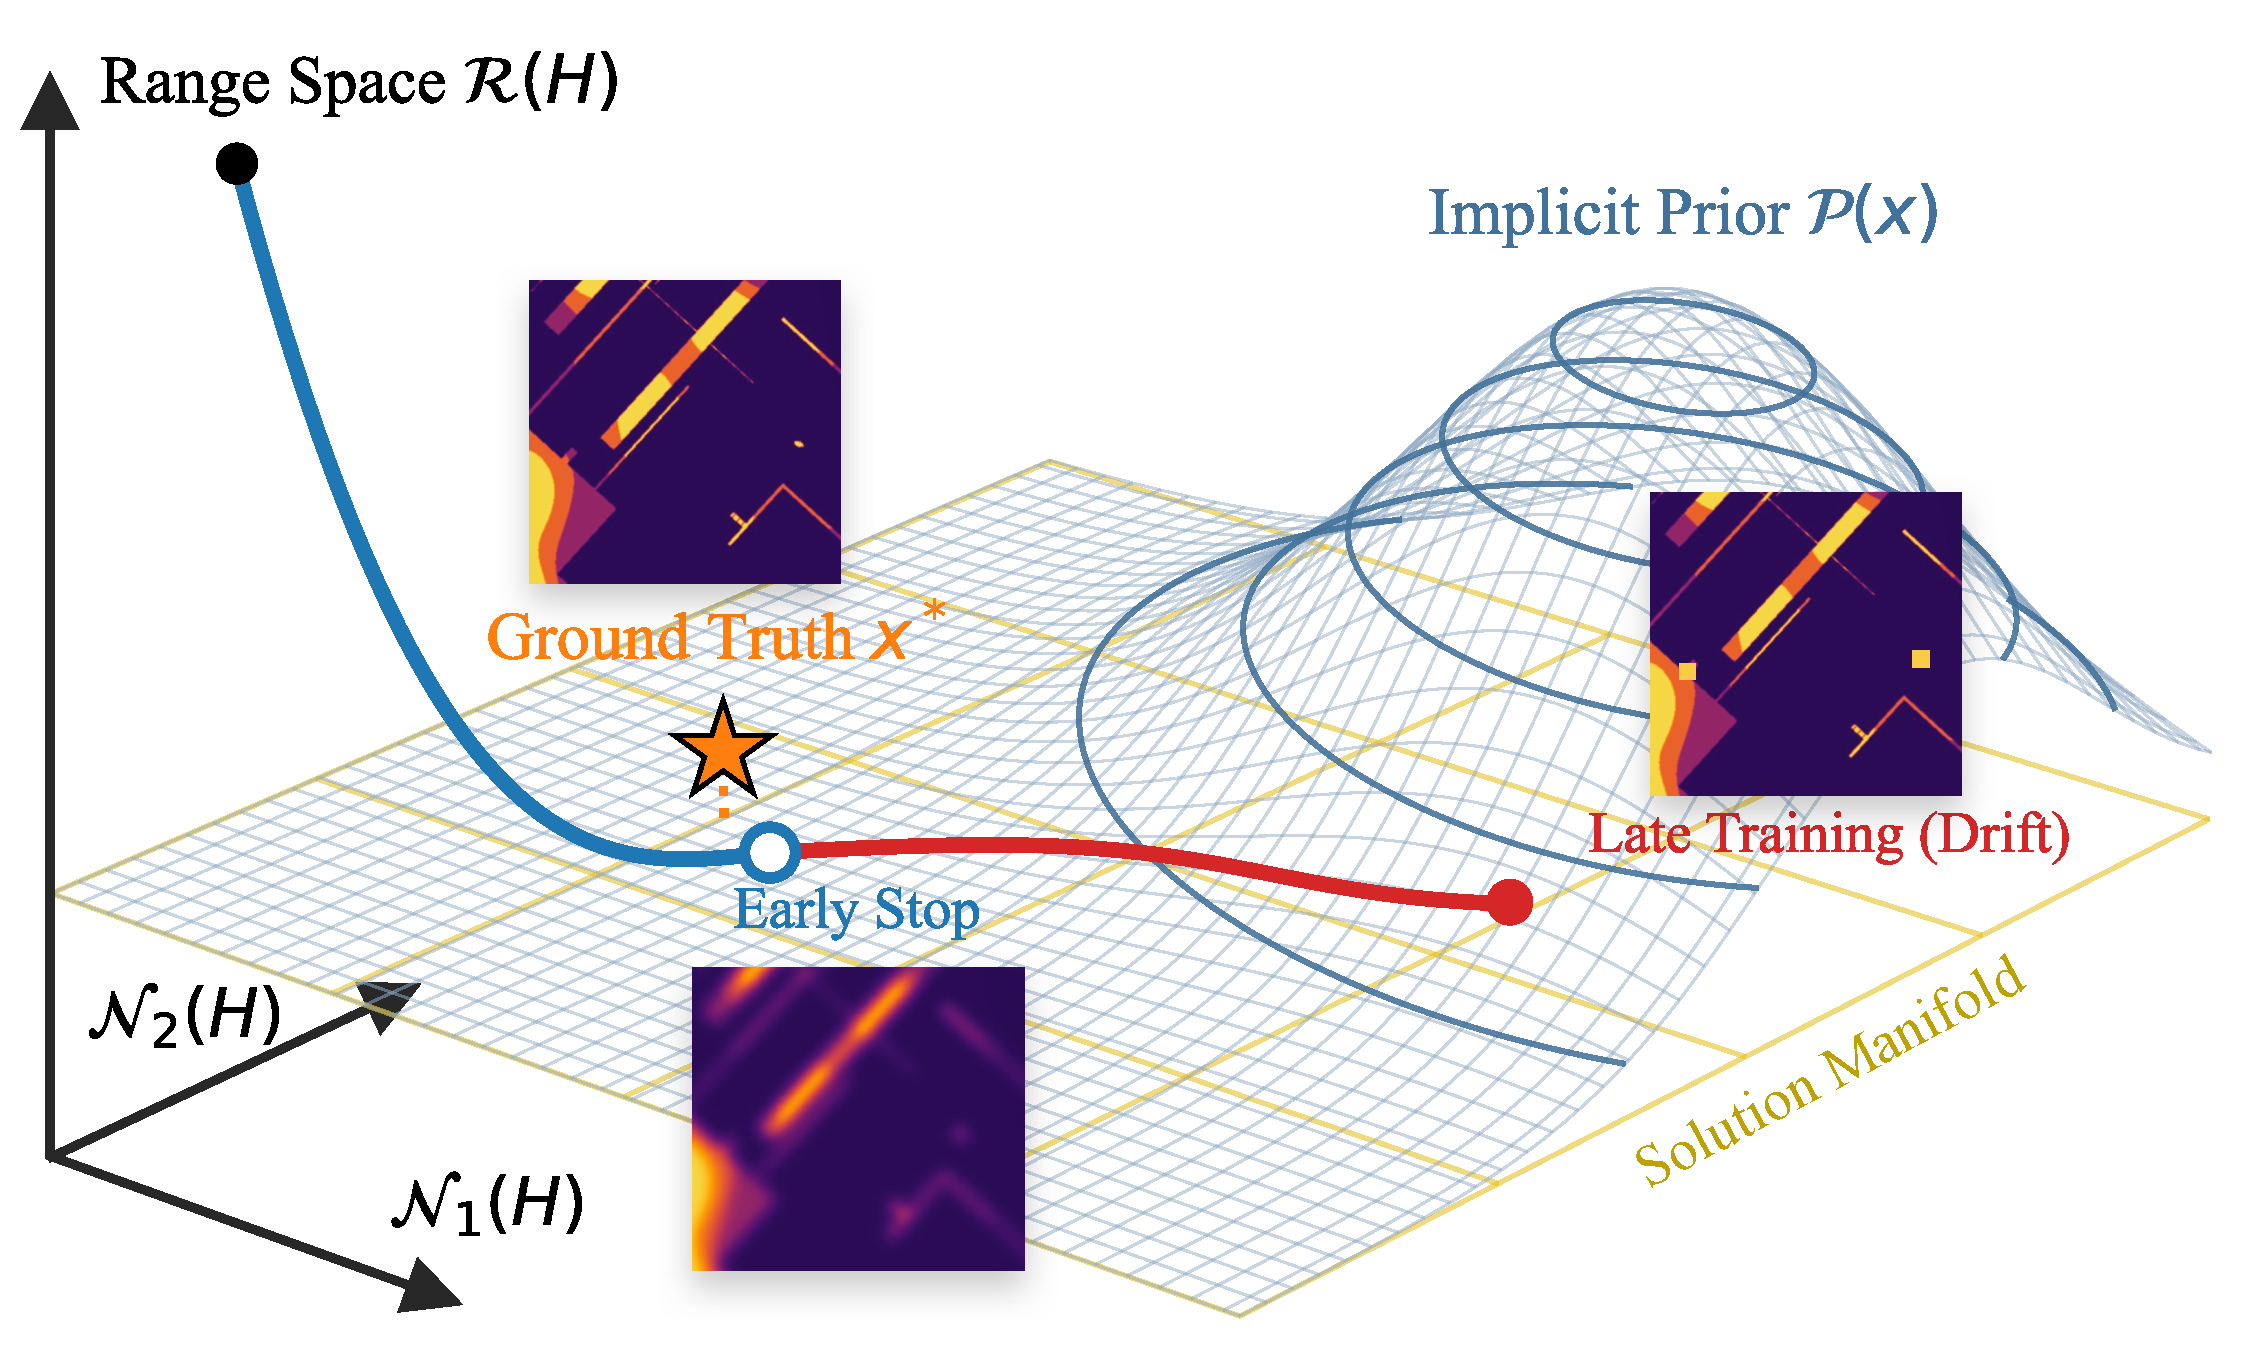
\includegraphics[width=0.95\linewidth]{../figures/fig_nullspace_drif.pdf}
  \caption{Null-space drift on real data. As training progresses, the model generates high-frequency artifacts consistent with the null/near-null space of the observation operator (artifact proxy rises) while data consistency (forward loss) remains at the noise floor.}
  \label{fig:teaser}
\end{figure}

Long-wave infrared (LWIR) thermography measures sub-degree temperature differences
arising from defects and process variations, and has become a key modality for
non-destructive semiconductor inspection \citep{breitenstein2010lockin}. In this
setting, inspection decisions are made directly from reconstructed images: spurious
structural features in the reconstruction can cause misdiagnosis rather than mere
blur. Yet the modality is constrained by both physics and data availability.
Optical systems are diffraction-limited, so spatial structure above the cutoff
frequency cannot be transmitted; higher-end optical solutions are costly with
limited gain; and paired high-resolution thermal ground truth required for
learning-based super-resolution is unavailable. The central question is therefore
whether multi-frame computational enhancement can substitute for hardware upgrades
to make internal chip contours reliably clearer on the existing instrument.

Micro-scanning provides the physical basis for this. A motorized stage translates
the scene in sub-pixel steps and acquires frames sequentially, yielding sub-pixel
phase diversity absent from a single frame---the standard setting of classical
multi-frame super-resolution \citep{tsai1984multiframe,farsiu2004fast}. This
setting comes with a fundamental difficulty, however: no high-resolution thermal
ground truth exists at any point during acquisition or deployment. There is no
paired HR sensor in this modality and scene; optical microscopy is not
radiometrically comparable and is not registered to the thermal camera.
Consequently, paired training data, full-reference evaluation metrics, and
validation-PSNR-based model selection---all relied upon by learning-based
SR---fail on real data.

In natural-image super-resolution and related domains, a common response to
missing paired ground truth is to train on synthetically degraded data and deploy
directly to the target domain, using sharper outputs as evidence of improvement
\citep{wang2021real,zhang2021designing}. In ground-truth-free settings, however,
``looking more detailed'' is precisely a failure mode rather than a success indicator
\citep{mittal2013making}. This risk is often called hallucination and is widely
recognized in the community, but rarely quantified systematically. Our goal is to
quantify this phenomenon, characterize its mechanism, and build a 2$\times$
contour-level enhancement pipeline that survives quantitative scrutiny.

We organize the paper around three progressive questions. First, does the
information exist: does the multi-frame observation sequence actually contain
recoverable information beyond single-frame resolution? We bound the coherent
information in the burst using phase-stratified split-half FRC with positive,
negative, and drift controls \citep{vanheel2005fourier}, and cash this margin into
a baseline floor that all learning methods must meet via a classical deconvolution
anchor. Second, is the information delivered: do learning models actually receive
sub-pixel phase information? A controlled comparison fixing network architecture
and loss while varying only the input representation shows that with conventional
per-frame statistical features, sub-pixel phase collapses at the input encoding
stage and the network cannot exploit it; only after injecting the same information
as a finer-grid drizzle channel does phase structure become visible in training.
Third, are added details faithful: is new detail anchored to the observations?
This is our central finding. Networks trained on synthetic data drift along the
null space of the observation operator on real data
\citep{schwab2019deep,chen2021equivariant}: forward-consistency loss stays at the
noise floor while artifact diagnostics on real data continue to worsen, and any
\emph{bounded} observation-domain anchor is blind to this drift component.
Effective remediation lies not in stronger consistency penalties but in
input-side evidence injection and mechanized checkpoint selection rules.

\textbf{Contributions.} This paper makes two contributions. (1) We identify and
characterize \textbf{null-space drift} in ground-truth-free thermal burst SR:
networks trained on physics-matched synthetic data, when transferred to real
data, show diagnostic evidence that newly added high-frequency detail is consistent
with null/near-null-space drift of the observation operator; combined with
fixed-operator null/near-null-space analysis (supp.\ A.2), bounded
observation-side anchoring cannot see this drift component, so effective remediation
requires input-side evidence injection---re-injecting sub-pixel phase via a
finer-grid drizzle channel. (2) Under a ground-truth-free evaluation protocol---phase-stratified split-half FRC with controls, observation-anchored proxy pairs, and mechanized checkpoint selection (supp.\ A.3--A.4, C.5), which provides only bounded proxy-level criteria rather than optical ground truth---we provide an \textbf{honest classical-vs-learning verdict}: classical variational reconstruction is most faithful on verifiable observation metrics, while learning reconstruction looks most detailed yet carries the most unverifiable high-frequency content, exhibiting complementary failure modes; with bounded criteria and no HR thermal ground truth, no single method is certifiably dominant.
